This section is intended for readers who are not already familiar with the power system. Will clarify basic concepts like production/consumption balance, system frequency, System Operators, Energy markets, etc.

The electric power system as it is today is composed of two layers (seen in Fig.~\ref{fig:powernow}-\ref{fig:marketnow}): 
\begin{description}
	\item[Market layer] This is where all the energy trade and business operations are made. This includes the sale of electricity from producers to balance responsible consumers (BRCs). Retailers in turn buy electricity from the BRCs and sell it to the end consumer. Being a Balance Responsible Party (BRP), either as a consumer or as a producer, means that the actor is responsible for its own forecasts and must ensure as best as possible that the actual production/consumption follows the planned schedules.
	\item[Physical grid] This is the level at which the electricity actually flows, going from generators to transmission system, to distribution system and finally to the end consumer.
\end{description}

\begin{figure}
	\centering
	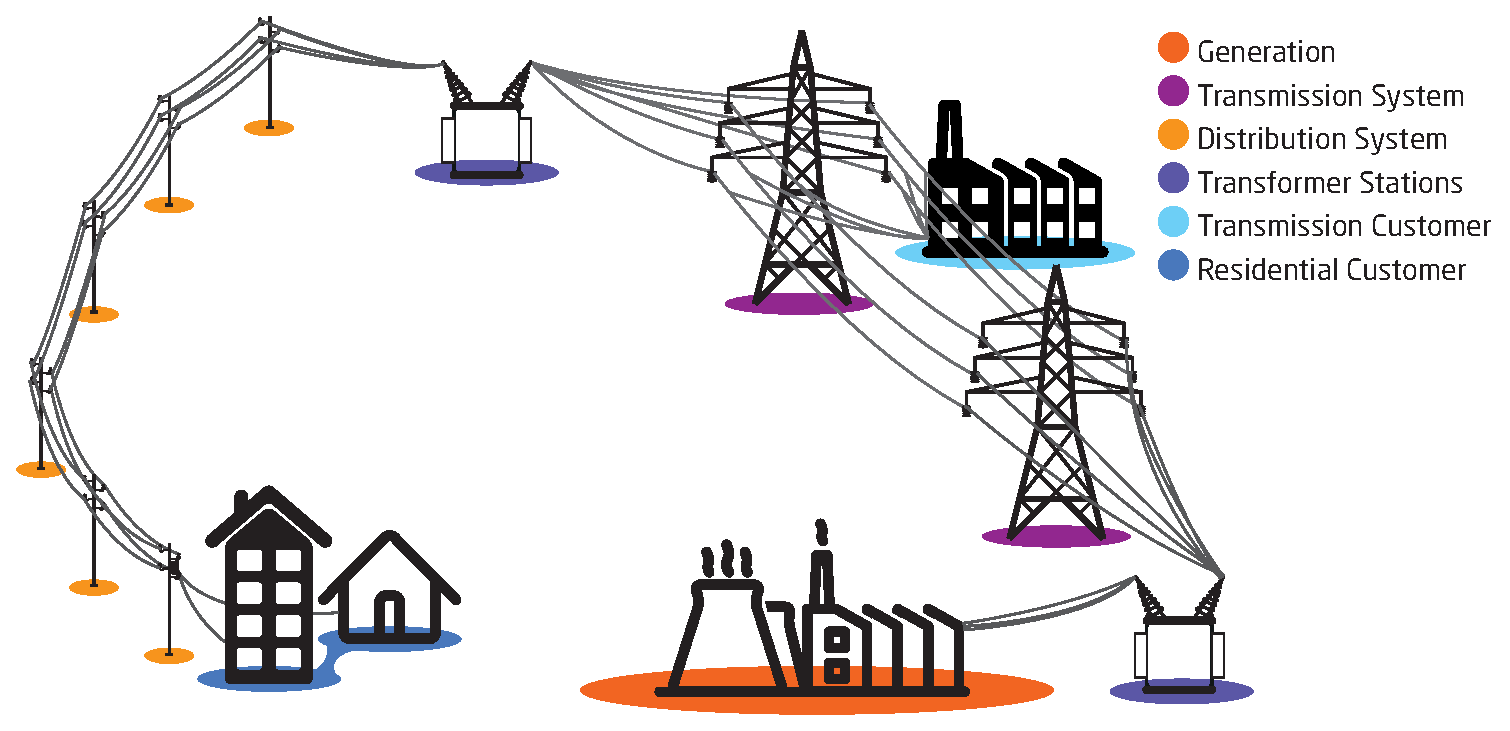
\includegraphics[width=\textwidth]{intro/traditional_grid.eps}
	\caption{The Electric Power System as seen today. The power generated is first transmitted at high voltage levels to substations, from where it is distributed at low voltage to medium size consumers and households.}\label{fig:powernow}
\end{figure}
\begin{figure*}
	\centering
	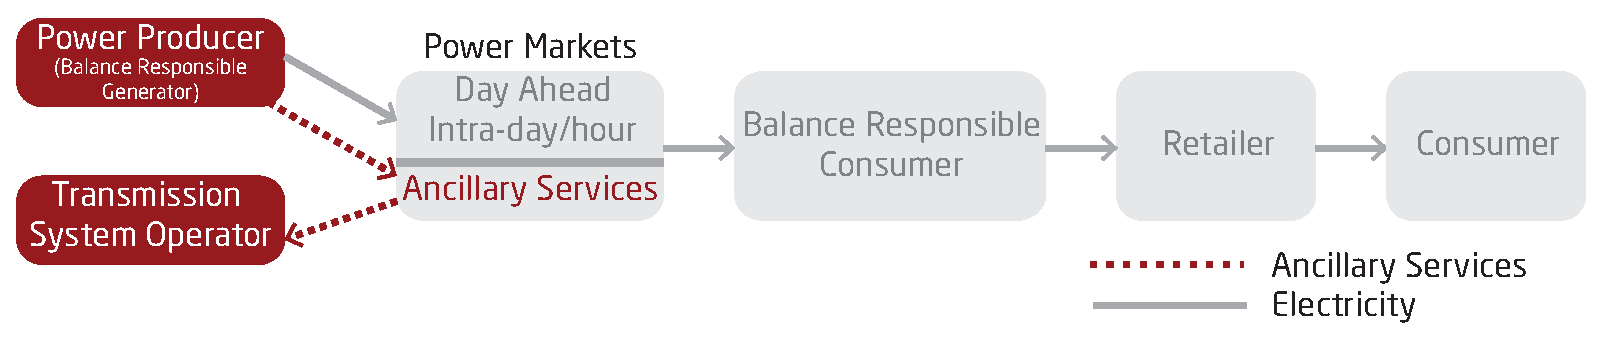
\includegraphics[width=\textwidth]{intro/market_now.eps}
	\caption{The actors and relationships in the power market today. Note that the consumer buys electricity from a retailer, but has no further contact to the other market actors.}\label{fig:marketnow}
\end{figure*}


While market regulations can be adjusted or completely changed in order to cope with the large influx of renewables, the physical laws cannot.
The fact is that when electricity is produced it must also somehow be consumed. With current technology it is unfeasible to store electricity in large quantities, therefore, electricity companies must make forecasts on how much electricity we (consumers) are going to need next day, and buy electricity accordingly. 

So, the production of electricity must match the consumption of electricity. If there is too much electricity in the system (production exceeds consumption), the frequency increases, and might eventually damage electric components in the grid. Vice versa, too little electricity in the system (consumption exceeds production) will cause a blackout. 

Since our forecasts are only relatively precise there will always be an unbalance between production and consumption. The Transmission System Operator (TSO) is the entity responsible of resolving the unbalances of the system. In order to do this, it buys ancillary services from the generators. This market relationship is also reflected in Fig.~\ref{fig:marketnow}. There are many different kinds of services, and [find a source listing the ancillary services, entsoe or sedc] gives a thorough overview of these. Here it suffices to say that for most ancillary services, the TSO will pay generators to deviate from their planned production plans in order to bring the system back to balance. In the future, we expect that the way the electric power system works will change.
